\chapter{Gas absorption}
 \label{sec:absorption}

\graphicspath{{Figs/abs/}}

\starthistory
  2013-06-21 & New intro and general revision. Added CIA part. --- Stefan Buehler\\
  2012-08-28 & Updated to propmat\_clearsky --- by Richard Larsson. \\
  2011-07-05 & Added intro and sections on abs in RT and abs
               calculation. Also revised lookup table section. First 
               attempt of a complete absorption
               chapter for ARTS2. --- Stefan Buehler\\
  2003-03-28 & Documentation for WSM abs\_fieldCalc
               extended by Stefan Buehler after comment from Sreerekha
               T.\ R.. \\
  2003-03-10 & Lookup tables added by Stefan Buehler.\\
  2002-06-04 & Restarted for ARTS-1-1 by Stefan Buehler.
\stophistory

\startsymbolswithunits
  \AbsCoef     & m$^{-1}$          &                          & Scalar gas absorption coefficient\\
  \Mpi         & $\frac{\mbox{W}}{\mbox{m$^2$ Hz sr}}$ & \wsvindex{iy}  & Intensity\\
  \PpathLng    & m                 &                         & Path length element\\
  \aDen{i}     & molec/m$^{-3}$          &                          & Number density of species $i$\\
  \aAbsXsec{i} & m$^2$/molec    & \wsvindex{abs\_xsec\_per\_species}    & Absorption cross-section of\\
&&&                                                               absorbing species $i$\\ 
  \aAbsXsec{i,j} & m$^5$/molec$^2$  & \wsvindex{abs\_cia\_data}         & Binary absorption cross-section of \\
&&&                                                              absorbing  species pair ($i$,$j$) \\ 
  \ExtMat      & m$^{-1}$ (4$\times$4) & \wsvindex{propmat\_clearsky}    & Clear-sky propagation matrix
 \label{symtable:absorption}     
\stopsymbolswithunits

\section{Introduction}

When calculating radiative transfer, the local absorption 
at each point in the atmosphere has to be known.  Furthermore, if one
also wants to calculate Jacobians, then the partial absorption
for different atmospheric components (different
absorption species) also has to be known.   

This chapter discusses different practical aspects of absorption in
ARTS. Sections \ref{sec:absorption:quantities} and
\ref{sec:absorption:agendas} introduce the main physical quantities
and the main agendas, respectively. Section
\ref{sec:absorption:abs-rt} explains how absorption is handled inside
radiative transfer calculations.  Section
\ref{sec:absorption:calculating} discusses how absorption is actually
calculated, and how the calculation is set up.  Finally, Section
\ref{sec:absorption:lookup} describes how absorption is stored in a
lookup table, and how it is extracted again.

Here in the User Guide we focus on practical aspects of absorption in
ARTS. But absorption calculations also have a deep theoretical
background, particularly the line-by-line calculations and the
continuum models.  Some of this background is discussed in \theory,
Chapter \ref{T-sec:abs_theory}. 


\section{Key physical quantities}
\label{sec:absorption:quantities}

The scalar gas absorption coefficient \AbsCoef\ has units of 1/m.  You
can think of it as being defined by the Lambert-Beer law
\begin{equation}
  \Mpi_1 = \Mpi_0 e^{-\AbsCoef \PpathLng},  
\end{equation}
where \Mpi\ is intensity and \PpathLng\ is the distance through a
homogeneous medium with absorption coefficient \AbsCoef.  

Absorption is additive, so the total absorption is the sum of the
partial absorptions of all absorbers.  For an individual absorber, we
can define another important quantity, the absorption cross-section
\aAbsXsec{i}, as
\begin{equation}
  \aAbsXsec{i} = \frac{\aAbsCoef{i}}{\aDen{i}},
\end{equation}
where subscript $i$ denotes the absorber and \aDen{i} is the partial
number density of that absorber.  Absorption cross-sections depend
less strongly on pressure than absorption coefficients, and are
therefore more suitable for storing in a lookup table.

Some processes create polarized absorption, which is described by a
4$\times$4 matrix, in ARTS called propagation matrix
(\wsvindex{propmat\_clearsky}, already introduced in Section \ref{sec:rteq}).  This variable is used by the ARTS RT
functions to describe absorption.  In the absence of polarizing
effects it is simply equal to $\AbsCoef \IdnMtr_4$, where $\IdnMtr_4$
is the 4$\times$4 identity matrix. 

Both, gases and particles in the atmosphere absorb, and the total absorption is
the sum of these two contributions.
This chapter only deals with absorption of non-scattering matter, i.e., gas
absorption in the first place (but can also include absorption by grey-body
particles and polarization changes by electrons).
%But this chapter is only about the gas absorption.

\section{Agendas}
\label{sec:absorption:agendas}

There are two key agendas related to absorption in ARTS:
\wsaindex{propmat\_clearsky\_agenda} and
\wsaindex{abs\_xsec\_agenda}.  They fulfill different purposes and
complement each other.  Agenda propmat\_clearsky\_agenda is called by
RT methods when they need absorption (more precisely the clear-sky
propagation matrix, as defined above). Hence, this agenda is the
interface between the RT part and the absorption part. Is is explained
further in the next section. 

The other agenda, abs\_xsec\_agenda, is called when absorption is
actually calculated (either inside propmat\_clearsky\_agenda, if
absorption is handled on-the-fly, or before, when the absorption
lookup table is generated).  This agenda is just for the scalar gas
absorption part and describes in detail the line-by-line absorption
calculation and various continua.  It is explained further in Section
\ref{sec:absorption:calculating}.  You will likely need both of the
above agendas for your ARTS RT simulation.


\section{Gas absorption in radiative transfer simulations}
\label{sec:absorption:abs-rt}

The interface between the RT part of ARTS and the
absorption part of ARTS is the agenda
\wsaindex{propmat\_clearsky\_agenda} (see Figure \ref{fig:absorption:pmat_outside}).  RT functions execute this
agenda whenever they need local absorption matrices.  In a typical
ARTS run, the agenda will be executed many times over, for different
points in the atmosphere.  See the built-in documentation for the
exact input and output arguments of the agenda.  The idea is that
input arguments are the local atmospheric conditions (temperature,
pressure, trace gas volume mixing ratios, magnetic field, etc.).

\begin{figure}
 \begin{center}
  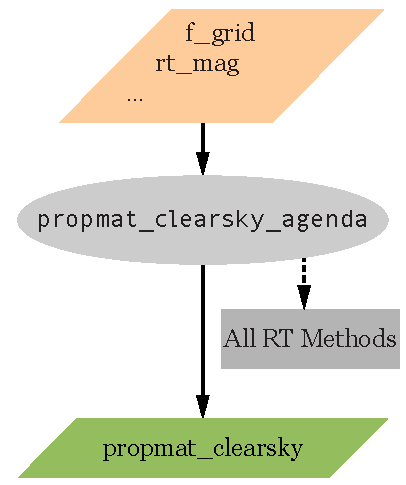
\includegraphics[scale=0.7]{propmat_clearsky_agenda}
  \caption{An outside view of propmat\_clearsky\_agenda.}
  \label{fig:absorption:pmat_outside}
 \end{center}
\end{figure}

The output of the agenda is a single variable,
\wsvindex{propmat\_clearsky}, a tensor with dimensions of absorption
species, frequency, Stokes dimension and Stokes dimension (Stokes
dimension of one thus emulates scalar absorption).  The physical
quantity corresponding to this variable is the clear-sky propagation
matrix \aAbsMat{a}\, as defined in Equation
\ref{eq:propmattotal}. It describes all non-scattering extinction
effects, that is, absorption and related polarization effects.

An inside view of propmat\_clearsky\_agenda is given in Figure
\ref{fig:absorption:pmat_inside}.  The agenda can contain a number of
different workspace methods that in some way or other compute
propmat\_clearsky. See the built-in documentation of the individual
methods to learn more. File \fileindex{agendas.arts}, one of the
standard include-controlfiles, predefines some typical alternatives
how propmat\_clearsky\_agenda can be set for different purposes.

\begin{figure}
 \begin{center}
  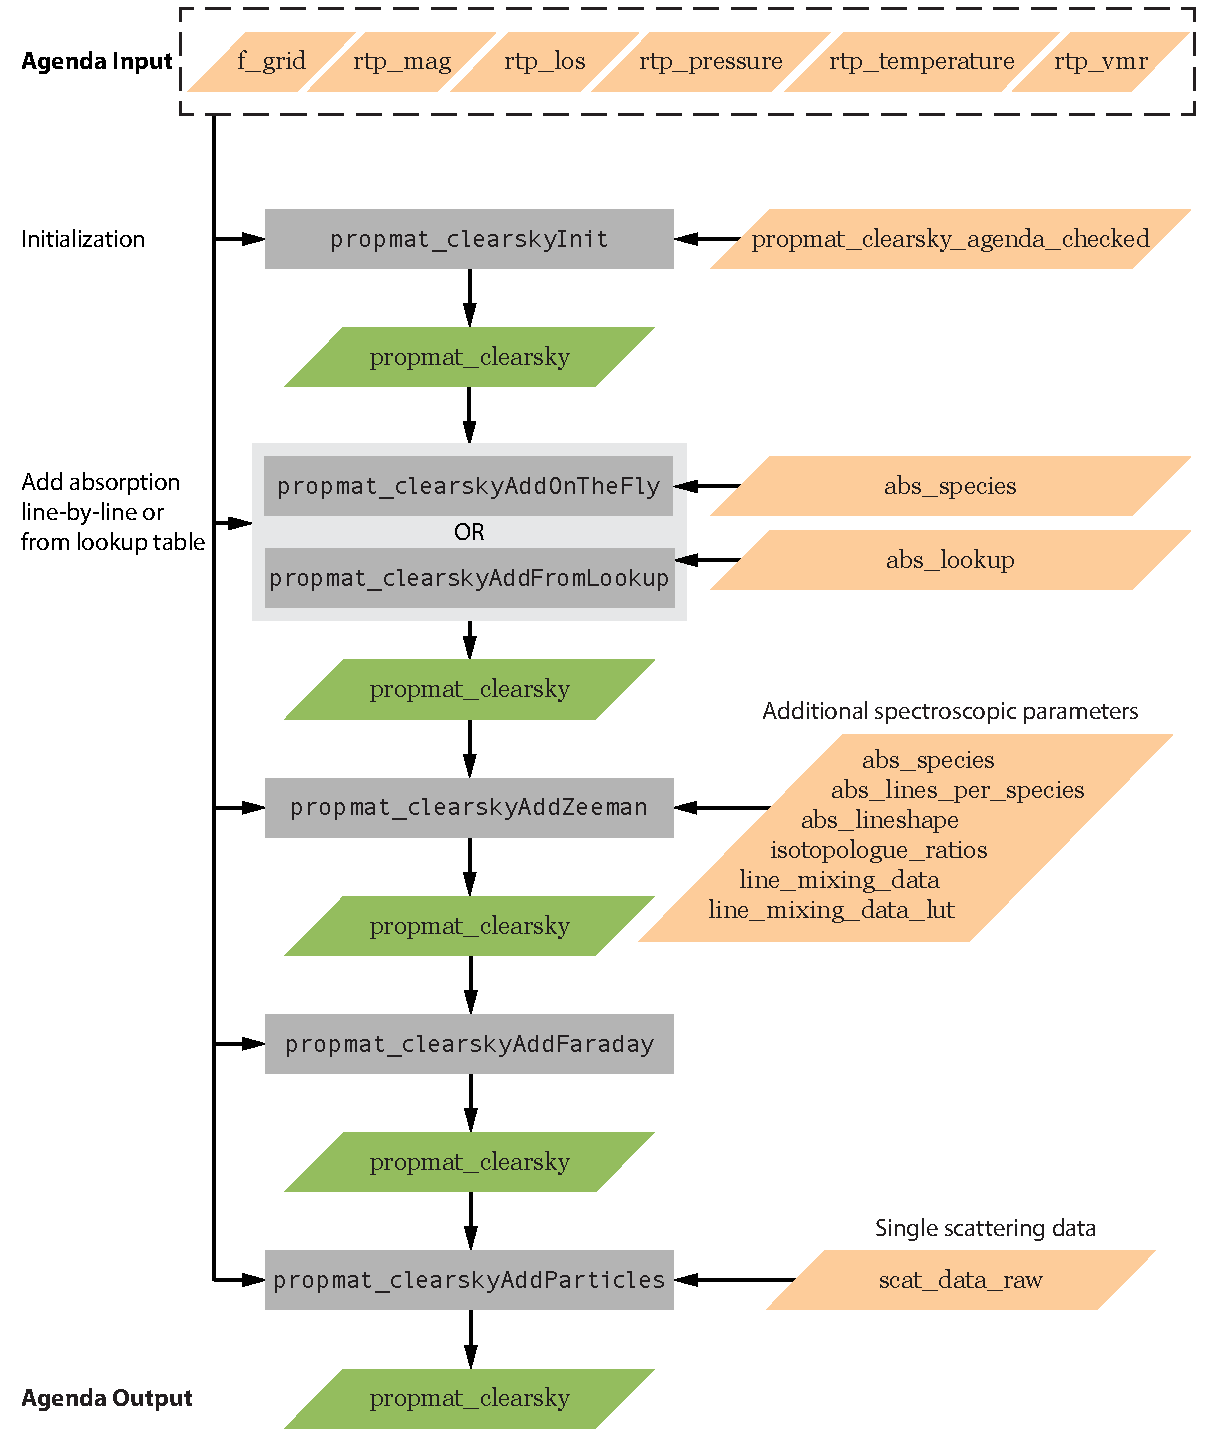
\includegraphics[scale=0.7]{propmat_clearsky_agenda_detail}
  \caption{An inside view of propmat\_clearsky\_agenda. At the same
    time, this gives an outside view of abs\_xsec\_agenda, as input to
    \wsmindex{propmat\_clearskyAddOnTheFly} in the context of
    on-the-fly absorption generation.}
  \label{fig:absorption:pmat_inside}
 \end{center}
\end{figure}



\section{Calculating gas absorption}
\label{sec:absorption:calculating}

This section deals with calculating gas absorption matrices in
ARTS.  This can typically occur in three different contexts:
as on-the-fly absorption matrix calculation within the radiative transfer
calculation,
% (see Section \ref{sec:absorption:abs-rt}), %this reference is more confusing than helping
when preparing
a gas absorption lookup table (see Section \ref{sec:absorption:lookup}),
or when the user is only interested in the absorption itself (see Section
\ref{sec:absorption:abs-only}).

In all these cases, the same agenda is used to actually calculate
absorption: abs\_xsec\_agenda. Outside views of this agenda are shown
in Figure \ref{fig:absorption:pmat_inside} (as input to
\wsmindex{propmat\_clearskyAddOnTheFly} in the context of on-the-fly
absorption generation) and Figure \ref{fig:absorption:xsec_in_lookup}
(as input to \wsmindex{abs\_lookupCalc} in the context of absorption
lookup table generation).

\begin{figure}
 \begin{center}
  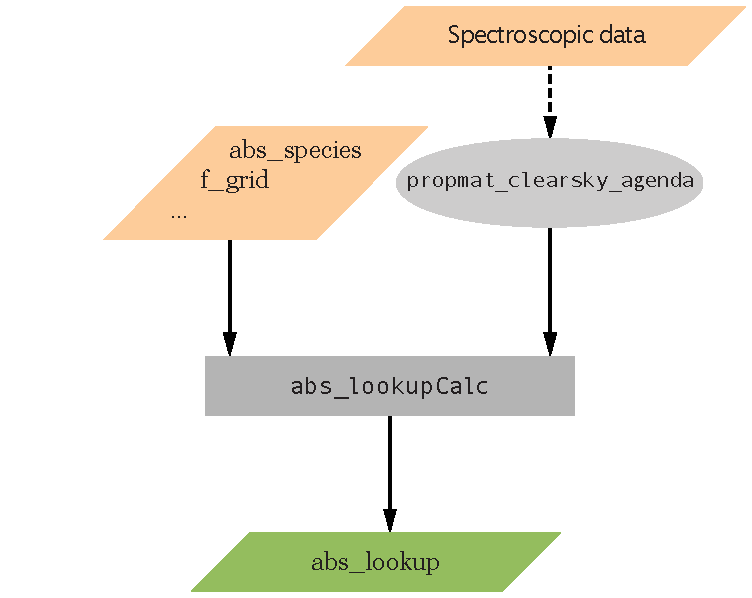
\includegraphics[scale=0.7]{abs_lookupCalc}
  \caption{An outside view of abs\_xsec\_agenda, in the context of
    absorption lookup table generation.}
  \label{fig:absorption:xsec_in_lookup}
 \end{center}
\end{figure}

An inside view of abs\_xsec\_agenda is given in Figure
\ref{fig:absorption:xsec_inside}.  The agenda can contain a number of
different workspace methods that in some way or other compute
abs\_xsec. See the built-in documentation of the individual methods to
learn more. As for propmat\_clearsky\_agenda, file
\fileindex{agendas.arts} predefines some typical alternatives also for
abs\_xsec\_agenda.

\begin{figure}
 \begin{center}
  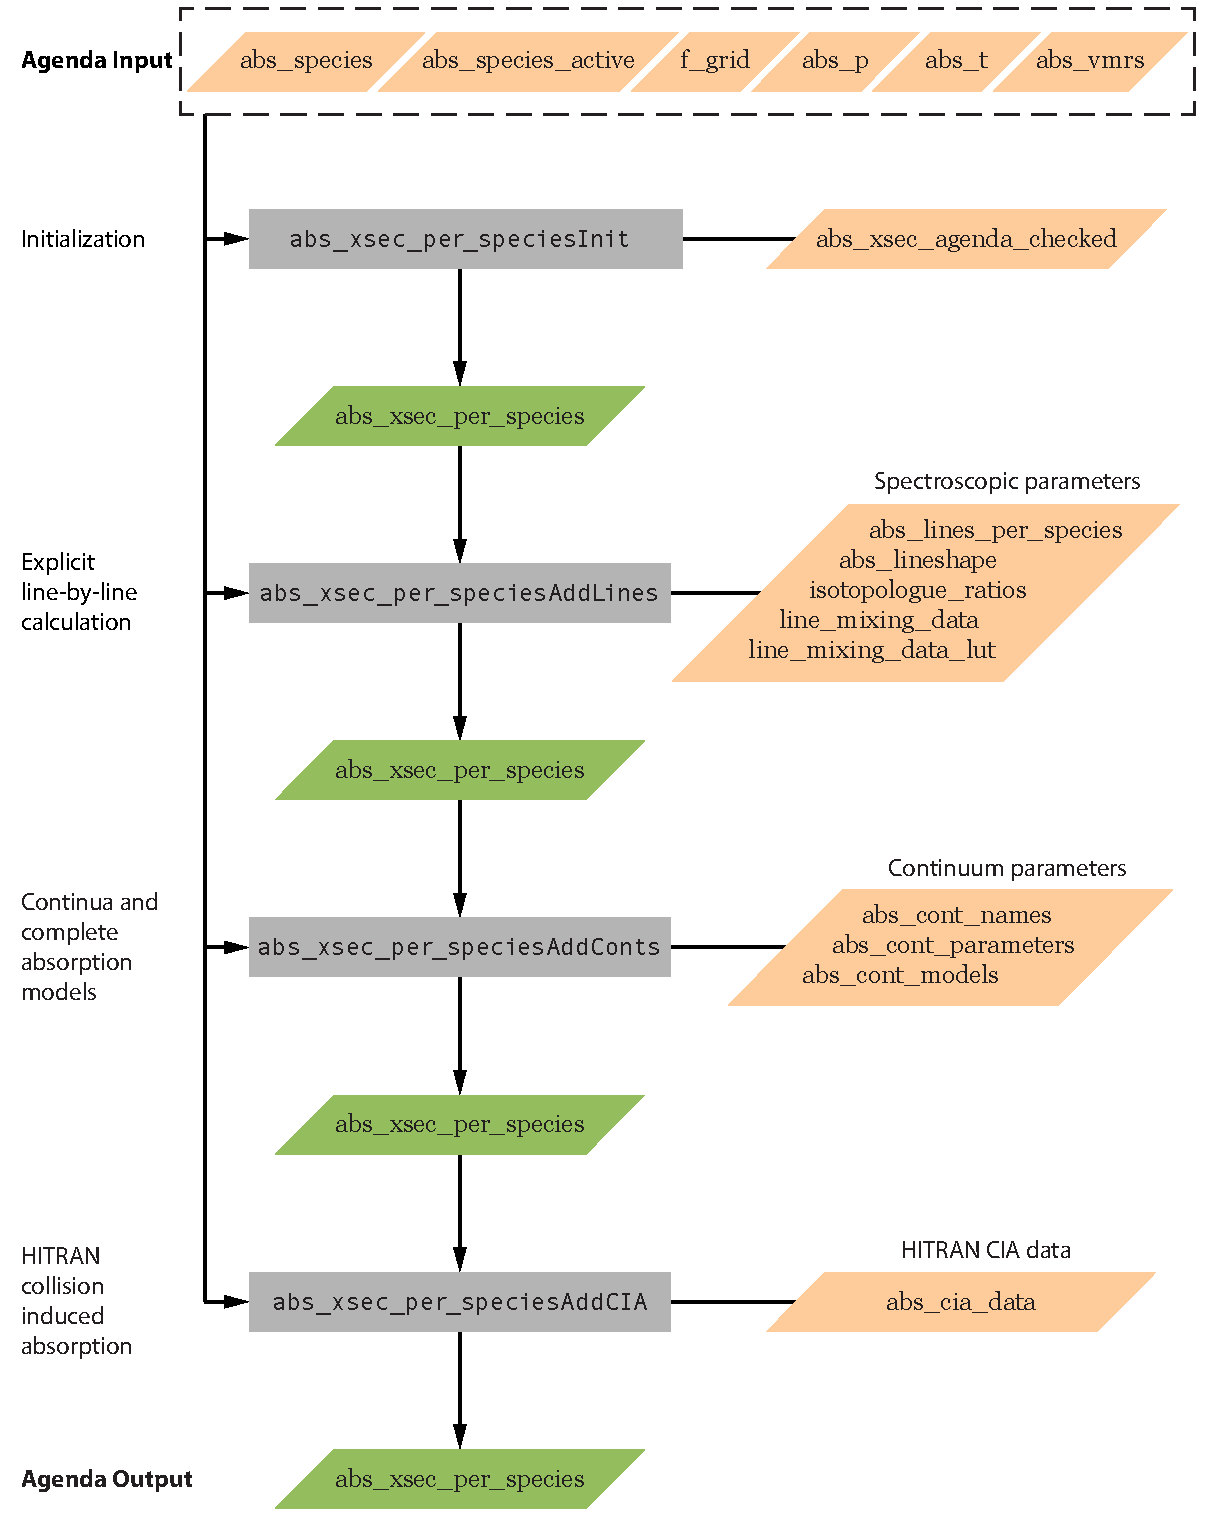
\includegraphics[scale=0.7]{abs_xsec_agenda}
  \caption{An inside view of abs\_xsec\_agenda.}
  \label{fig:absorption:xsec_inside}
 \end{center}
\end{figure}


\subsection{Absorption species}

Absorption is additive, so the total absorption is simply the sum of
all partial absorptions.  And the partial absorption for gases that
have spectral lines can be calculated as a sum over the absorption of
each spectral line, plus some more or less empirical continuum terms.

An absorption species in ARTS is an abstract entity that has a partial
absorption matrix associated with it, and that usually can be
associated with a volume mixing ratio of a corresponding gas (the VMRs
are stored in variable \wsvindex{vmr\_field}). Total absorption is the
sum of the partial absorptions of all absorption species. Absorption
species are defined in the ARTS controlfile by special `tags', which
are stored in the variable \wsvindex{abs\_species}, and set by the
method \wsmindex{abs\_speciesSet}.

The absorption species tags specify the different considered absorbers, which can
be gaseous species but also free electrons and (grey-body) particles.
For gaseous species, they also describe the model that should be used to
calculate the absorption for each of the species.
There are three types of tags, those for explicit line-by-line
calculations, those for continua and complete absorption models, and a special
Zeeman effect tag.
An example of the first kind is \verb|"H2O-18"|, which identifies a
particular isotopologue of water vapor. An example of the second kind is
\verb|"H2O-ForeignContCKDMT100"|, which identifies a particular continuum
model. An example of the third is \verb|"O2-Z"|, which identifies that special Zeeman
routines should be used.
Tags can be combined, if they refer to the same molecule
(different isotopologues are allowed). Even continuum tags can be combined
with explicit line-by-line tags, if they refer to the same molecule.

It should be noted that isotopologue ratios are taken into account
implicitly when line strengths are calculated, so even if you make
calculations for individual isotopologues, the VMR numbers in the
variable \wsvindex{vmr\_field} should not be adjusted for the isotopologue
ratio (the isotopologue ratio can be changed instead; see
Section~\ref{sec:absorption:isoratio}). As an example, to make a line-by-line
calculation for all ozone isotopologues, you could represent them in different
ways by
\wsmindex{abs\_speciesSet}.
\begin{code}
a) abs_speciesSet(species=["O3"])
b) abs_speciesSet(species=
                  ["O3-666, O3-668, O3-686, O3-667, O3-676"])
c) abs_speciesSet(species= 
                  ["O3-666", "O3-668", "O3-686", "O3-667", "O3-676"])
\end{code}
Options (a) and (b) are equivalent, you will have one ozone species
that represents all isotopologues, and that will be associated with a
single VMR field in \wsvindex{vmr\_field}.  With option (c) you have
five different ozone species, so you have to supply five different VMR
fields. If those five fields are identical (exactly same numerical
values), you will get the same total absorption as with options (a)
and (b).

Overall, the tag mechanism allows quite complex absorption setups. The built-in
documentation for \wsmindex{abs\_speciesSet} gives a detailed explanation of the
tag syntax and some examples.

Particularly note, that order of the species list matters as absorption line
data is assigned to species in their order within the \wsvindex{abs\_species}
list and no line record is assigned to more than one species.
It is furthermore important to note that there is no `intelligence' in ARTS that
checks that the chosen tag combinations make sense, so the user should
know what s/he is doing, or follow one of the many examples in
the ARTS \fileindex{controlfiles} directory.

\subsection{Explicit line-by-line calculations}

For absorption species with explicit line-by-line calculation the
calculation involves the steps summarized in Table
\ref{tab:absorption:lbl}, which contains the steps that are common to all the
three contexts in which explicit line-by-line calculations can occur as well
as the steps that are specific to each of those cases. 
The list of variables and methods in the
table is not complete. The idea is to give an overview over the
important ones and show how they work together. Missing are
particularly the input variables that describe the atmospheric
conditions, and continuum description variables, which normally do not
have to be set by the user anyway.

\begin{table}
\footnotesize
\renewcommand{\arraystretch}{1.5}
\newcounter{rownum}
\newcommand{\mylabel}[1]{\refstepcounter{rownum} \label{#1}}
\begin{tabularx}{\hsize}{l>{\raggedright\arraybackslash\hsize=0.5\hsize}X
                          >{\raggedright\arraybackslash\hsize=1.5\hsize}X}
\hline
\# & Step & Variables and Methods \\
\hline
%---------------------------------------------------------------------
\mylabel{step:lineshape}
\arabic{rownum} & 
Define line shape function(s) to use. &
Variable:
\wsvindex{abs\_lineshape}. \newline
Methods:
\wsmindex{abs\_lineshapeDefine} (same shape for all species),
\wsmindex{abs\_lineshape\_per\_tgDefine} (different shapes for different
species). \\
%---------------------------------------------------------------------
\mylabel{step:readline}
\arabic{rownum} &
Read spectral line data (the order of the first two steps does not
matter). &
Variable: \wsvindex{abs\_lines}. \newline
Methods: 
\wsmindex{abs\_linesReadFromArts},
\wsmindex{abs\_linesReadFromSplitArtscat},
\wsmindex{abs\_linesReadFromHitran},
\wsmindex{abs\_linesReadFromHitranPre2004},
\wsmindex{abs\_linesReadFromJpl},
\wsmindex{abs\_linesReadFromMytran2} (different methods are for
different catalogue formats). For the ARTS internal format, the
standard method \wsmindex{ReadXML} works also, but does not allow to
select a frequency range, as the others do. \\
%---------------------------------------------------------------------
\mylabel{step:splitline}
\arabic{rownum} &
Split line data for different absorption species. &
Variable: \wsvindex{abs\_lines\_per\_species}. \newline
Methods:
\wsmindex{abs\_lines\_per\_speciesCreateFromLines}. Alternatively, read
lines from different catalogues for different species directly with
\wsmindex{abs\_lines\_per\_speciesReadFromCatalogues}. \\
%---------------------------------------------------------------------
\mylabel{step:optline}
\arabic{rownum} &
Optimize line data. (optional)&
Variable: \wsvindex{abs\_lines\_per\_species}. \newline
Methods: Add mirror lines for VVW line shape with
\wsmindex{abs\_lines\_per\_speciesAddMirrorLines} (see \theory,
Chapter \ref{T-sec:abs_theory}). Remove lines that are outside the
line shape cutoff with \wsmindex{abs\_lines\_per\_speciesCompact}. \\
%---------------------------------------------------------------------
\multicolumn{3}{>{\raggedright\arraybackslash\hsize=2\hsize}X}{The
  first four steps are preparation, and typically 
  have to be done only once per ARTS run. The fifth step is the actual
  absorption calculation, which can occur in different contexts.} \\
%---------------------------------------------------------------------
\mylabel{step:calc}
\arabic{rownum}a &
Calculate absorption on-the-fly. &
Agenda: \wsaindex{propmat\_clearsky\_agenda}. \newline
Variable: \wsvindex{propmat\_clearsky}, which is nitialized in \wsmindex{propmat\_clearskyInit}.\newline
Methods: \wsmindex{propmat\_clearskyAddOnTheFly} (the core method for on-the-fly
absoprtion calculation inlcuding line-by-line and continuum absorption), \newline
\wsmindex{propmat\_clearskyAddZeeman} (see Sec.~\ref{sec:absorption:zeeman}), \newline
\wsmindex{propmat\_clearskyAddFaraday} (see Sec.~\ref{sec:absorption:faraday}), \newline
\wsmindex{propmat\_clearskyAddParticles} (see Sec.~\ref{sec:absorption:particles}). \newline
Alternative:
\wsmindex{propmat\_clearskyAddFromLookup} instead of \wsmindex{propmat\_clearskyAddOnTheFly}
(extract absorption from pre-calculated lookup table, see
Sec.~\ref{sec:absorption:lookup}). Note that the lookup
table cannot contain absorption for Zeeman tagged species, Faraday rotation, and
particles due to their directional dependencies.\\
%---------------------------------------------------------------------
\arabic{rownum}b &
Calculate absorption lookup table. &
Variable: \wsvindex{abs\_lookup}. \newline
Methods: \wsmindex{abs\_lookupCalc}. Alternative: Load lookup table
from file with \wsmindex{ReadXML}, it then has to be adapted to the
current calculation (and checked) with \wsmindex{abs\_lookupAdapt}. \\ 
%---------------------------------------------------------------------
\arabic{rownum}c &
Calculate absorption only (no RT). &
Variable: \wsvindex{propmat\_clearsky\_field}, \wsvindex{abs\_coef}. \newline
Methods, high level: \wsmindex{propmat\_clearsky\_fieldCalc}. \newline
Methods, low level: \newline
\wsmindex{abs\_xsec\_per\_speciesInit}, \newline
\wsmindex{abs\_xsec\_per\_speciesAddLines} (the core method for the
actual line-by-line calculation, used internally by all higher level methods),\newline
\wsmindex{abs\_xsec\_per\_speciesAddConts} (add continua or complete absorption
models, see Section \ref{sec:absorption:continua}),\newline
\wsmindex{abs\_xsec\_per\_speciesAddCIA} (add collision induced absorption, see
Section \ref{sec:absorption:cia}),\newline
\wsmindex{abs\_coefCalcFromXsec} (calculate absorption coefficients
from absorption cross-sections). \\
%---------------------------------------------------------------------
\hline
\end{tabularx}
\caption{Steps for line-by-line absorption calculation, and associated
    ARTS workspace variables and methods.}
\label{tab:absorption:lbl}
\end{table}

See the built-in documentation of the various variables and methods
for more information.  It is on purpose not repeated here, for better
maintainability.  If you are viewing this pdf file on a computer, just
click on a variable or method name to get to the corresponding
built-in documentation. Further input data and parameters required (not only)
for line-by-line calculations is described in Section~\ref{sec:absorption:input}.

\subsection{Continua and complete absorption models}
\label{sec:absorption:continua}

ARTS includes many absorption continua and complete absorption models,
which are described in \theory, Chapter \ref{T-sec:abs_theory}.  The
common property of all of these is that they do not use the standard
ARTS line-by-line calculation mechanism.  They may include spectral
lines, but then these lines are hardwired into the absorption model
itself.  Consequently, the first four steps in Table
\ref{tab:absorption:lbl} are not needed for these models.  

The pure continua are intended to be used together with an explicit ARTS
line-by-line calculation, the complete models are intended to be used alone.
To select a continuum or complete absorption model, simply use the
corresponding tag with \wsmindex{abs\_speciesSet}.  Currently available
models are listed in Table \ref{tab:absorption:continua}.

\begin{table}
\centering
\footnotesize
\begin{tabular}{ll}
\hline  
Class & Tag name \\
\hline  
%---------------------------------------------------------------------

Water vapor continua
& H2O-SelfContStandardType \\
& H2O-ForeignContStandardType \\
& H2O-ForeignContMaTippingType \\
& H2O-ContMPM93 \\
& H2O-SelfContCKD222 \\
& H2O-ForeignContCKD222 \\
& H2O-SelfContCKD242 \\
& H2O-ForeignContCKD242 \\
& H2O-SelfContCKD24 \\
& H2O-ForeignContCKD24 \\
& H2O-SelfContCKDMT100 \\
& H2O-ForeignContCKDMT100 \\
& H2O-SelfContCKDMT252 \\
& H2O-ForeignContCKDMT252 \\
& H2O-ForeignContATM01 \\[1ex]

Complete water vapor models
& H2O-CP98 \\
& H2O-MPM87 \\
& H2O-MPM89 \\
& H2O-MPM93 \\
& H2O-PWR98 \\[1ex]

Carbon dioxide continua 
& CO2-CKD241 \\
& CO2-CKDMT100 \\
& CO2-CKDMT252 \\
& CO2-SelfContPWR93 \\
& CO2-ForeignContPWR93 \\
& CO2-SelfContHo66 \\
& CO2-ForeignContHo66 \\[1ex]

Oxygen continua 
& O2-CIAfunCKDMT100 \\
& O2-v0v0CKDMT100 \\
& O2-v1v0CKDMT100 \\
& O2-visCKDMT252 \\
& O2-SelfContStandardType \\
& O2-SelfContMPM93 \\
& O2-SelfContPWR93 \\[1ex]

Complete oxygen models & O2-PWR98 \\
& O2-PWR93 \\
& O2-PWR88 \\
& O2-MPM93 \\
& O2-MPM92 \\
& O2-MPM89 \\
& O2-MPM87 \\
& O2-MPM85 \\
& O2-TRE05 \\[1ex]

Nitrogen continua & N2-SelfContMPM93 \\
& N2-SelfContPWR93 \\
& N2-SelfContStandardType \\
& N2-SelfContBorysow \\
& N2-CIArotCKDMT100 \\
& N2-CIAfunCKDMT100 \\
& N2-CIArotCKDMT252 \\
& N2-CIAfunCKDMT252 \\
& N2-DryContATM01 \\[1ex]

Condensate absorption models & liquidcloud-MPM93 \\
& icecloud-MPM93 \\
& rain-MPM93 \\

%---------------------------------------------------------------------
\hline  
\end{tabular}
\caption{ARTS continua and complete absorption models. The molecular
  species can be inferred from the start of the tag name.  See
  \theory, Chapter \ref{T-sec:abs_theory} for more information on the
  various models.}
\label{tab:absorption:continua}
\end{table}

The names should be fairly self-explanatory and can be used to find
background information on the various models in \theory.  The
condensate absorption models are a bit special and perhaps need some
extra explanation. They are absorption parameterizations by Liebe, and
allow the inclusion of condensate in the (rare) cases where scattering
is not important. Their general applicability is therefore fairly limited.

The behavior of the continua and complete absorption models can be
modified by passing them some additional parameters, stored in the
variables \wsvindex{abs\_cont\_names}, \wsvindex{abs\_cont\_models},
and \wsvindex{abs\_cont\_parameters}. Basically,
\builtindoc{abs\_cont\_names} identifies the model,
\builtindoc{abs\_cont\_models} contains switches that select different
behavior (for example taking only the lines, or only the continuum
part of a complete model), and \builtindoc{abs\_cont\_parameters} can
contain numerical parameters. 

Yes, the nomenclature for these additional continuum parameters,
particularly \builtindoc{abs\_cont\_models}, is confusing. However,
most users will never have to deal with these variables
explicitly. They are set to default values in the include file
\fileindex{continua.arts}. Users should therefore always include this file  at
the start of their controlfiles with
\begin{code}
  INCLUDE "continua.arts"
\end{code}
Unless you work on continuum model development or verification, you
should never have to modify these default settings.

The core method to calculate continua and complete absorption models
is \wsmindex{abs\_xsec\_per\_speciesAddConts}.  Users normally do not
have to call this method explicitly, since it is used implicitly by
higher level methods, such as \wsmindex{propmat\_clearskyAddOnTheFly} and
\wsmindex{propmat\_clearsky\_fieldCalc}.

\subsection{Collision-induced absorption}
\label{sec:absorption:cia}

Collisions of molecules centro-symmetric molecules, e.g., \chem{O_2},
\chem{N_2}, \chem{H_2}, \chem{CO_2}, and \chem{CH_4}, possessing no permanent
electric dipole create a transient dipole, which causes so-called collision-induced
absorption (CIA). Absorption strength of CIA is characterized by its dependency
on the molecular density of both molecular species involved in the collision.

Recently, the well-known HITRAN spectral line catalogue has started to
offer also tabulated binary absorption cross-sections for CIA.  This is
described in detail in \citet{richard:12}, and also in the documentation that
comes with the data themselves.

Binary absorption cross-sections
\aAbsXsec{i,j} have to be multiplied with the number densities of both involved
molecular species to yield absorption coefficients:
\begin{equation}
\aAbsCoef{i,j} =  \aAbsXsec{i,j} \, \aDen{i} \, \aDen{j},
\end{equation}
where $i$ and $j$ denote the two different absorbing species. As a
consequence, \aAbsXsec{i,j} has units of m$^5$/molec$^2$ in ARTS (the
original HITRAN units are different).

Using CIA in ARTS is easy. First of all, include one or more CIA tags
in your absorption species list (\wsvindex{abs\_species}). All valid
tags are listed in Table \ref{tab:absorption:cia_ranges}. Secondly,
read in WSV \wsvindex{abs\_cia\_data}, which contains the tabulated
binary absorption cross-sections, from a file. This will usually be the
file \fileindex{hitran\_cia2012\_adapted.xml.gz}, which is included in the
\shortcode{arts-xml-data}, but the original HITRAN data files can also be
read. Finally, use WSM \wsmindex{abs\_xsec\_per\_speciesAddCIA} in
abs\_xsec\_agenda to add the CIA absorption. For usage examples, look
in directory \fileindex{controlfiles/artscomponents/cia} that is part
of the ARTS distribution.

Figure \ref{fig:absorption:cia} shows all CIA continua that are
currently available in ARTS (left) and separately the ones that are
relevant for Earth's atmosphere (right). The valid frequency and
temperature ranges for these data, as available in ARTS, are listed in
Table \ref{tab:absorption:cia_ranges}. Outside the covered frequency ranges, the
binary absorption cross-sections are set to zero, while exceeding the valid
temperature range will produce \verb|NaN| values and eventually trigger a
runtime error.

To make the HITRAN data work in ARTS, some modifications were necessary,
specifically:

\begin{description}
\item[N$_2$-N$_2$:] The two high-frequency datasets were merged into one.
\item[O$_2$-O$_2$:] Three apparently separate datasets that really
  belong together were merged. UV/Vis dataset were removed.
\item[CO$_2$-CO$_2$:] Caveat: This is only the self continuum of
  CO2. The CO2-air continuum has strong features above 250\,cm$^{-1}$ that
  are present in CKD\_MT (also available in ARTS as one of the
  continuum and full absorption models), but are missing here.
  %The HITRAN data also generally looks weird. It is only in the alternative
  %folder, and \citet{richard:12} basically recommend not to use it. Conclusion:
  %No changes, but usage not recommended.
  Furthermore, \citet{richard:12} point out that for molecules with more than two atoms
  further mechanisms affecting CIA exist, which are not covered by the simple
  models used. They hence state that ``these data should be used very
  carefully''. Conclusion: No changes, but use with care.

  Also note that no data exists at frequencies below 30\,GHz (1\,cm$^{-1}$)
  though some significant absorption is still present at the limiting frequency.
  For those low frequencies, the CO2-SelfContPWR93 continuum (see
  Table~\ref{tab:absorption:continua}) can be used as an alternative (we
  estimated that to be valid at least up to about 100\,GHz, but deviating
  significantly above 500\,GHz).
\item[O2-N2, O2-CO2:] These UV/Vis-only datasets were removed.

\begin{table}
    \caption{Absorption species tags, frequency ranges, and
      temperature ranges for HITRAN CIA data as implemented in
      ARTS. (These data contain some modifications from the original
      HITRAN data, which are described in the text.)} 
    \label{tab:absorption:cia_ranges}
    \centering
    \begin{tabular}{llll}
\hline
    CIA tag& Spectral range [cm$^{-1}$]& Temp range [K]& No. of datasets\\
\hline
  N2-CIA-N2-0& 0.02 -- 554.00& 40.00 -- 400.00& 10\\
  N2-CIA-N2-1& 1850.00 -- 3000.09& 228.20 -- 362.50& 10\\
  N2-CIA-H2-0& 0.02 -- 1886.00& 40.00 -- 400.00& 10\\
  N2-CIA-CH4-0& 0.02 -- 1379.00& 40.00 -- 400.00& 10\\
  H2-CIA-H2-0& 20.00 -- 10000.00& 200.00 -- 3000.00& 113\\
  H2-CIA-He-0& 20.00 -- 20000.00& 200.00 -- 9900.00& 334\\
  H2-CIA-CH4-0& 0.02 -- 1946.00& 40.00 -- 400.00& 10\\
  H2-CIA-H-0& 100.00 -- 10000.00& 1000.00 -- 2500.00& 4\\
  He-CIA-H-0& 50.00 -- 11000.00& 1500.00 -- 10000.00& 10\\
  O2-CIA-O2-0& 1150.00 -- 1950.00& 193.40 -- 353.40& 15\\
  CO2-CIA-CO2-0& 1.00 -- 250.00& 200.00 -- 800.00& 7\\
  CH4-CIA-CH4-0& 0.02 -- 990.00& 40.00 -- 400.00& 10\\
  CH4-CIA-Ar-0& 1.00 -- 697.00& 70.00 -- 296.00& 5\\
\hline
\end{tabular}
\end{table}


\end{description}

\begin{figure}
 \begin{center}
  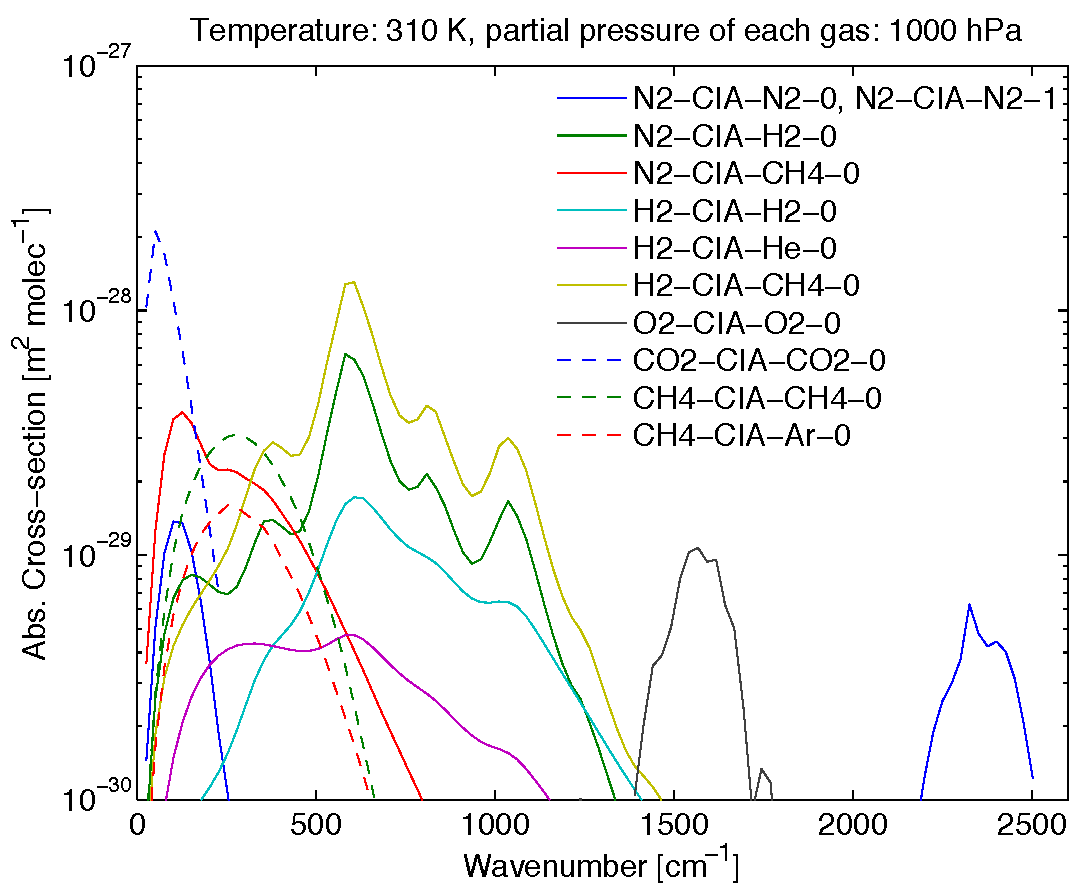
\includegraphics[width=.46\hsize]{plot_all_arts_cia_generic_1}
  \hspace{\fill}
  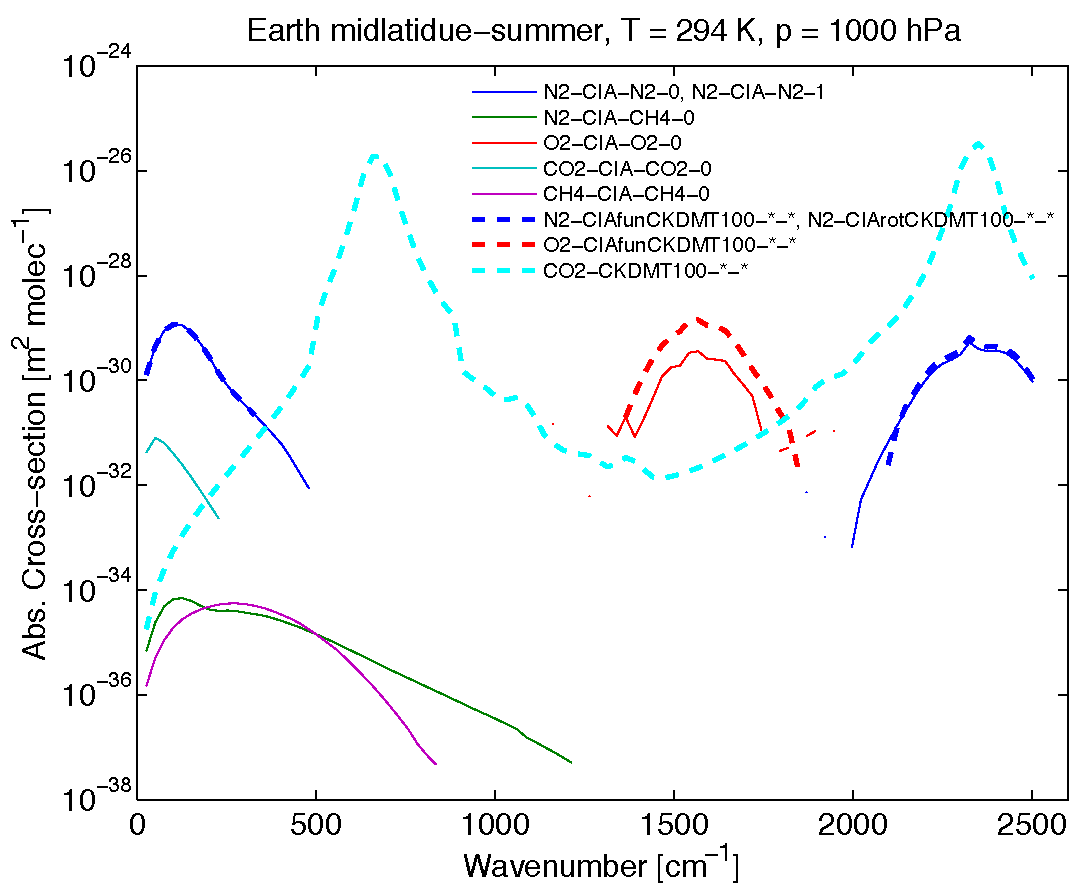
\includegraphics[width=.46\hsize]{plot_earth_continua_1_1}
  \caption{Left: All HITRAN CIA continua that are implemented in ARTS
    (each gas here has a partial pressure of 1000\,hPa). Right: Only
    the ones that are relevant for Earth (for Earth surface
    conditions).}
  \label{fig:absorption:cia}
 \end{center}
\end{figure}

\subsection{Zeeman calculations}
\label{sec:absorption:zeeman}

The Zeeman effect is calculated in the method \wsmindex{propmat\_clearskyAddZeeman}.
If this method is included in the \builtindoc{propmat\_clearsky\_agenda}, then species with the
tag "\verb|-Z|" will be calculated as Zeeman species. If the method is not included,
then these species will simply be ignored. Note that the order within the tag
string is important: the Zeeman tag must directly follow the molecular species
tag. That is, \verb|O2-Z-66| will be counted as Zeeman splitting on the
O$^{16}$O$^{16}$ molecule, whereas \verb|O2-66-Z| will not work the same way, or even at all.

The physics and internal workings of the Zeeman calculations follow the scheme
presented in \citet{larsson:xx} %FIXME: update bibtex reference when accepted.
%Larsson et al., submitted 2013 to JQSRT, \textit{A treatment of the Zeeman
%effect using Stokes formalism and its implementation in the Atmospheric
%Radiative Transfer Simulator ARTS}.

In order to calculate Zeeman splitting, additional line parameters that are not
readily available in, e.g., HITRAN are necessary. These include $g_s$ [-], the
relative Land\'{e} factor, and $S$ [-], the molecular total spin. These
variables must therefore be read to the WSV \wsvindex{isotopologue\_quantum}.
This variable is of type \builtindoc{SpeciesAuxData}, and a file providing
that kind of data would, e.g., look like:
\begin{code}
<arts format="ascii" version="1">
  <SpeciesAuxData version="1" nelem="1" nparam="3">
    @ O2-66 2.002064 1 1
  </SpeciesAuxData>
</arts>
\end{code}
In this example, \verb|@| indicates the beginning of a new data record, \verb|O2-66|
specifies what isotopologue is associated with the data, the number
\verb|2.002064| is the relative Land\'{e} factor, and the molecule got $S=1$.
The last value indicates what Hund case is used in the calculations. For oxygen,
Hund case b is used, indicated b the number "1". Presently, Hund case a, indicated
by number "0" also works for some molecules. It is up to the user to assure the
correct quantum numbers for each case are set properly.
The supported molecules in ARTS so far for Zeeman calculations are
\begin{itemize}
\item O$_2$, case b
\item NO, case a/b
\item OH, case a
\item ClO, case a
\item HO$_2$, case b
\item NO$_2$, case b
\end{itemize}
but only O$_2$ is tested beyond initial modeling results.

Beside the additional line parameters, it is also necessary to input the magnetic
field into the model. This can be done following:
\begin{code}
GriddedField3Create(B)
  ReadXML(B,"B_1comp.xml.gz")
  GriddedFieldLatLonRegrid( B, lat_grid, lon_grid, B )
  GriddedFieldPRegrid( B, p_grid, B )
  FieldFromGriddedField( mag_w_field, p_grid, lat_grid, 
                         lon_grid, B )
\end{code}
where \verb|B_1comp.xml.gz| contains the (atmospheric) profile or field for one
components of the magnetic field. 
Since the magnetic field is usually not dependent on the pressure,
it is also possible to use the  
\begin{code}
 GriddedFieldZToPRegrid(*)
\end{code}
functionality to input altitude-gridded magnetism.
Input needs to be provided for each non-zero
magnetic field component separately into the respective WSVs \wsvindex{mag\_w\_field}, 
\wsvindex{mag\_v\_field}, and \wsvindex{mag\_u\_field}. For more information on
magnetic field format in ARTS see Section~\ref{sec:atm:vecfields}.

Lastly, it is necessary to take phase effects into account when calculating the
Zeeman effect. It is therefore important that \wsvindex{abs\_lineshape} is
chosen such that it allows for this information to be provided. One
suitable line shape can be defined through
\begin{code}
abs_lineshapeDefine( abs_lineshape, "Faddeeva_Algorithm_916", 
                     "VVH", 750e9 )
\end{code}

\subsection{Internal line-mixing}
\label{sec:absorption:line-mixing}

Line mixing is implemented as the \verb|-LM-| species tag.  Added to 
a species, ARTS knows that it should look for lines with
line mixing data attached to them when it calculates the spectral cross sections.
Note that each line is initialized without any line mixing data, and with a tag 
state that says they are not to be line mixed.  If this is not changed before the
absorption calculations are performed, the line will regardless of species tag still
act like if it were not line mixed.  Also note that it is possible to calculate line mixing
in conjuncture with the Zeeman effect, but that it is not possible to calculate the line mixing
of individual Zeeman lines, which as far as we know when writing this is unimportant.

The possible tags on species \verb|X| that activates the line mixing module are thus
\verb|X-LM-*|, and \verb|X-Z-LM-*|.
The supported ways to ensure that the line record contains information on
how to calculate line mixing, thus not ignoring it, are 
\begin{itemize}
 \item Read an ARTS catalogue file with line mixing parameters.
 \item Read LBLRTM line catalogue containing line mixing parameters using 
 \verb|abs_linesReadFromLBLRTM(*)|.
 \item Read a line database that does not have line mixing, but use the 
 \verb|line_mixing_dataMatch(*)| method to inject line mixing data into the line record.
\end{itemize}
There is no preferred method in ARTS --- each work the same when they reach the absorption
calculations --- but we urge the user to be sure that line mixing data and the line database
are of the same origin, as the calculations will be of poor quality if this is not the case.

Example control file meta flow for code calculating line mixing using \verb|abs_linesReadFromLBLRTM|:
\begin{code}
# Define your atmospheric species,
abs_speciesSet(species=["O2-Z-LM","CO2-LM"])

# read from a line database,
abs_linesReadFromLBLRTM(filename="aer", 
    fmin=1e1,fmax=1e20)
\end{code}
Note that this meta flow is very similar to using an ARTS catalogue with line mixing.
These methods are easy, because they identity what line mixing method will be used 
directly from the catalogue.
It should be noted that LBLRTM also gives the non-resonant term of the molecular oxygen
spectra as a low frequency line.  If it is desired to calculate this term, the lower
frequency range must contain the line as per the definition of our reading routines.

Example control file meta flow for code calculating line mixing using \verb|line_mixing_dataMatch|:
\begin{code}
# Define your atmospheric species,
abs_speciesSet(species=["O2-Z-LM","CO2-LM"])

# Read from a line database,
abs_linesReadFromHITRAN(filename="HITRAN2012.par", 
    fmin=1e1,fmax=1e20)

# Sort the line records into the format ARTS wants
abs_lines_per_speciesCreateFromLines

# Create a way to temporally store O2 line mixing data.
ArrayOfLineMixingRecordCreate(lm_o2)
ReadXML(lm_o2,"o2.xml")

# Create a way to temporally store CO2 line mixing data.
ArrayOfLineMixingRecordCreate(lm_co2)
ReadXML(lm_co2,"co2.xml")

# Match the line mixing data with O2 and Zeeman effect
line_mixing_dataMatch(
    species_tag="O2-Z-LM",
    line_mixing_records=lm_o2
    line_mixing_tag=LM*)

# Match the line mixing data with O2 and Zeeman effect
line_mixing_dataMatch(
    species_tag="CO2-LM",
    line_mixing_records=lm_co2,
    line_mixing_tag=LM*)
\end{code}
The latter method is much more complicated than reading directly from the catalogue.
This is because the user has to ensure what type of line mixing is going on
and then parse that data properly to ARTS.  In order for ARTS to know what line the user 
wants to line mix, a series of line database matching 
based on the quantum numbers of the line is necessary.
This means that it only works for those species and catalogue formats
for which we have implemented quantum number reading.
This list is small but growing, and if you need help adding another species, 
let us know via the mailing list.

There are three \verb|line_mixing_tag| supported at this point:
\verb|"LL"|, \verb|"NR"| and \verb|"L2"|.  These refer to LBLRTM, and second order line mixing.
Setting these tags will tell ARTS how to calculate the line mixing of any particular line.
The data is matched from \verb|ArrayOfLineMixingRecord|,
which must contain a \verb|SpeciesTag|, a
\verb|QuantumNumberRecord|, and a vector that is the correct length for the method selected

Example of correct input data for using the second order approach ("L2"):
\begin{code}
<?xml version="1.0"?>
<arts format="ascii" version="1">
<Array type="LineMixingRecord" nelem="38">
<LineMixingRecord>
<SpeciesTag>"O2-66-*-*"</SpeciesTag>
<QuantumNumberRecord>
<Upper><QuantumNumbers nelem="3"> 
  J 1/1 N 1/1 v1 0/1 
</QuantumNumbers></Upper>
<Lower><QuantumNumbers nelem="3"> 
  J 2/1 N 1/1 v1 0/1 
</QuantumNumbers></Lower>
</QuantumNumberRecord>
<Vector nelem="10">
2.65e-06
-1.32e-07
-8.35e-12
8.43e-13
0.000545
0.00017
300
0.8
1.6
1.6
</Vector>
</LineMixingRecord>
</Array>
</arts>
\end{code}
The format of the above data is thusly: \shortcode{SpeciesTag},
\shortcode{QuantumNumberRecord}, \shortcode{Vector}, 
The above input will cause the \verb|O2-66-*-*| line with
upper quantum numbers $J=1$, $N=1$ and $\nu_1=0$ and with
lower quantum numbers $J=2$, $N=1$ and $\nu_1=0$ to match.
If this is the only input file, the described line is the only
line experiencing line mixing in your calculations. If there
were more lines in the file, these would also experience line mixing.
In order of appearance in the vector, its format is 
first order zeroth phase correction [Pa$^{-1}$], 
first order first phase correction [Pa$^{-1}$],
second order zeroth absorption correction [Pa$^{-2}$],
second order first absorption correction [Pa$^{-2}$],
second order zeroth line-center correction [Hz Pa$^{-2}$],
second order first line-center correction [Hz Pa$^{-2}$],
standard temperature for corrections [K],
first order phase temperature correction exponential term [-],
second order absorption temperature correction exponential term [-], and
second order line-center temperature correction exponential term [-].
The format of the vector is fixed according to necessary information found 
in \citet{makarov11:_60-ghz_jqsrt},
the naming scheme of the variables above can also be understood from the same work.
Note that first order line mixing, as per the MPM/PWR complete oxygen models, 
can be achieved with the correct input by letting the second order terms be nil.



Example of correct input data for using the LBLRTM approach ("LL" and "NR"):
\begin{code}
<?xml version="1.0"?>
<arts format="ascii" version="1">
<Array type="LineMixingRecord" nelem="38">
<LineMixingRecord>
<SpeciesTag>"O2-66-*-*"</SpeciesTag>
<QuantumNumberRecord>
<Upper><QuantumNumbers nelem="3"> 
  J 1/1 N 1/1 v1 0/1 
</QuantumNumbers></Upper>
<Lower><QuantumNumbers nelem="3"> 
  J 2/1 N 1/1 v1 0/1 
</QuantumNumbers></Lower>
</QuantumNumberRecord>
<Vector nelem="12">
200
250
296
340
-0.004433034295584e-4
-0.003982500863558e-4
-0.003628075993092e-4
-0.003341074759437e-4
0
0
0
0
</Vector>
</LineMixingRecord>
</Array>
</arts>
\end{code}
In this format, the first four values are a temperature grid in Kelvin.
For "LL" the following four values are the first order
line mixing coefficients at these temperature grid points [in units 1/Pa], 
and the last four are the second order line mixing coefficients at these temperature grid points [in units 1/Pa$^2$].
For "NR" the following four values are the first order
non-resonant term at these temperature grid points [in units 1/Pa], 
and the last four are the second order non-resonant terms
at these temperature grid points [in units 1/Pa$^2$].
ARTS will use linear interpolation to get proper coefficients between and slightly outside grid points.

\textit{Warning:} There appears to be some errors in the quantum number encoding
in HITRAN04 and HITRAN08 that makes the line mixing module wrong.  The newer
HITRAN2012 has fixed these issues.

\subsection{Faraday rotation}
\label{sec:absorption:faraday}

Faraday rotation is a change of polarization state of radiation in interaction
with (free) electrons in presence of a static magnatic field. For further
details on theory and usage in ARTS see Section~\ref{sec:faraday}.
Here we only give a short summary how to setup the calculation of Faraday
contribution to the absorption (or better: propagation) matrix
\wsvindex{propmat\_clearsky}.

First, to include Faraday rotation effects
\wsmindex{propmat\_clearskyAddFaraday} must be included in the
\builtindoc{propmat\_clearsky\_agenda}. Second, a species tag
\verb|"free_electrons"| needs to be contained in \wsvindex{abs\_species}.
Correspondingly, a field of electron densities is required in
\builtindoc{vmr\_field}.

For usage examples, check \fileindex{controlfiles/artscomponents/faraday} that
is part of the ARTS distribution.

\subsection{Absorbing particles}
\label{sec:absorption:particles}

% what are particles doing here? what for / when is this useful?
As pointed out before, this chapter deals with absorption by non-scattering
matter. In first place this refers to gases, while particles (aerosols, clouds,
precipitation) are considered to (also) scatter radiation and are handled
differently (see Chapters~\ref{sec:clouds}, \ref{sec:scattering:doit}, and
\ref{sec:scattering:mc}).
However, when particles are small compared to the wavelength of the radiation
they act as broadband grey-body absorbers and can be treated similarly to
continuum absorption by gases.

This is reflected in ARTS providing a few continuum models for condensed
matter (see Tab.~\ref{tab:absorption:continua}), which essentially are
particles, too.
It is tedious, though, to implement those kind of particle continua for a wide
range of different base materials as become of interest when being interested in
other than the Earth's atmosphere.

% concept (using scat_data/pnd_field-type data exists - make use of that)
In the ARTS scattering modules, particles are represented by single scattering
property data (\builtindoc{scat\_data}) and particle concentrations
(particle number densitity fields \builtindoc{pnd\_field}).
% These data usually originate from scattering theory (e.g., Mie theory,
% T-matrix model, Discrete dipole approximation) convolved with size
% distribution models and veetical and horizontal concentration distribution
% information.
The single scattering data originate from scattering theory
programs (e.g., Mie theory, T-matrix model, Discrete Dipole Approximation) and
their preparation typically requires significant efforts. Comprehensive data for
hydrometeors in the Earth atmosphere, but also clouds, dust and the like for
other planets is available from the \shortcode{arts-xml-data} package.
It is appealing to apply this data in non-scattering calculations (e.g. at low
frequencies, where the scattering contribution is negligible) in a consistent
manner. The ARTS method for that is \wsmindex{propmat\_clearskyAddParticles} and
its application is described in the following.

% how to setup
% - per particle type one "particle" tag in abs_species
% - corresponding pnd field into vmr_field
% - one entry per particle type into scat_data_single
% - (directional dependent absorption, polarized absoprtion)
To consider grey-body particle absorption, the user has to include
\wsmindex{propmat\_clearskyAddParticles} in the
\builtindoc{propmat\_clearsky\_agenda}. Furthermore, for each scattering element
(see Section~\ref{sec:clouds:intro} for how a scattering element is defined) 1) a
\verb|"particles"| tag needs to be added to \builtindoc{abs\_species}, 2) the
corresponding concentration field has to be added to \builtindoc{vmr\_field},
and 3) its single scattering data have to be added to
\wsvindex{scat\_data}. This can be done each-by-each using
\builtindoc{ReadXML} and \builtindoc{Append} methods, but a dedicated method
\wsmindex{ParticleType2abs\_speciesAdd} is available performing these three
steps for one scattering element at once. \wsmindex{ParticleType2abs\_speciesAdd}
adds the raw number density field to \builtindoc{vmr\_field\_raw}, i.e., the raw
concentration fields can be converted to internal atmospheric grids together
with the gas concentration fields using, e.g., \builtindoc{AtmFieldsCalc}.
Single scattering data of all individual scattering elements is added to one and
the same scattering species, specifically to the last one of these in the
\builtindoc{scat\_data} array.
Note that \wsmindex{ParticleType2abs\_speciesAdd} is essentially doing the same
as \builtindoc{ParticleTypeAdd}, but for non-scattering instead for
scattering-in-cloudbox cases (where in non-scattering setups the concentration
data is stored together with gas concentrations in \builtindoc{vmr\_field},
while for scattering setups it is stored separately in
\builtindoc{pnd\_field}), and that for the single scattering data and
concentration fields the exact same data can be applied.

% caveats: not to be used together with cloudbox - it's either or.
% plus/pro: in contrast to particles as continuum model, it consiers direction
% dependent and polarized absorption as occuring e.g. for non-spherical particles.
Beside being able to re-use particle data from scattering cases, this method is
also advantageous compared to the particles-as-continuum-models implementations
as it allows for directional dependent absorption and for polarization effects
that occur, e.g., with non-spherical particles.

Be aware that both \wsmindex{propmat\_clearskyAddParticles} and the scattering methods
use \wsvindex{scat\_data} to store the particle single scattering data.
Hence, it is straight-forward that these methods can not be applied
simultaneously. In one ARTS run, all particles are handled either as scattering
entities (when using the scattering modules) or as grey-body absorbers (when
applying \wsmindex{propmat\_clearskyAddParticles}). Trying to use both in
parallel results in a runtime error.

For a setup example check \fileindex{TestAbsParticle.arts} in
\fileindex{controlfiles/artscomponents/absorption/}. See the built-in
documentation of the individual methods for further information.


\subsection{Further input data and parameters for calculating gas absorption}
\label{sec:absorption:input}

\subsubsection{Spectral line data}
\label{sec:absorption:linecat}

Important input to the line-by-line calculations is the spectral line data,
usually provided by spectroscopic catalogues. ARTS has its own format for the
spectral line data, but is also capable of handling data from other catalogues
like HITRAN (both pre- and post-2004 formats) and JPL (see Table
\ref{tab:absorption:lbl}, step \ref{step:readline}).
Section~\ref{T-sec:abs_theory:catalogue_formats} of \theory\ contains more
information on the internal format of the spectral line data.  It also contains
theoretical background for the calculation itself.

\subsubsection{Isotopologue ratios}
\label{sec:absorption:isoratio}

Isotopologue ratios (mostly) from HITRAN and valid for Earth atmosphere are
stored in ARTS source code. These data is necessary for working with HITRAN data
(as HITRAN line strengths are weighted with isotopologue abundance). However,
it is convenient for the user to be able to change isotopologue ratio values,
e.g., when modeling absorption in other planets' atmospheres.

The WSV \wsvindex{isotopologue\_ratios} holds the isotopologue ratios applied in
the absorption calculation. They have to be set by the user. It is possible to
apply the ARTS built-in values mentioned above using
\wsmindex{isotopologue\_ratiosInitFromBuiltin}. Alternatively, they can be read
from file using \builtindoc{ReadXML}. For easy manipulation, the user might
initialize \wsvindex{isotopologue\_ratios} from built-in data, write the
\wsvindex{isotopologue\_ratios} structure to file using \builtindoc{WriteXML},
modify the data accordingly, and read in the manipulated file.
Files with isotopologue ratios for a couple of planetary atmospheres are
provided with the \shortcode{arts-xml-data} package.

It shall be noted, that only isotopologue ratios of the species used in the
absorption calculation need to be given. Reading in from file resets the full
list of isotopologue ratios (i.e., the values for all absorption species known to
ARTS) with species not given in the input data set to \verb|NaN|.

\subsubsection{Partition functions}
\label{sec:absorption:partition}

Partition functions are currently still hard-coded into ARTS. That is, no
settings related to those have to be or can be done on the user level. For more
information on theoretical background as well as the source and implementation
in ARTS see Section \ref{T-sec:abs_theory:species_data} of \theory.


\section{The gas absorption lookup table}
\label{sec:absorption:lookup}

\subsection{Introduction}

Calculating gas absorption matrix spectra in a line by line way
is quite an expensive thing to do. Sometimes contributions from
thousands or ten thousands of lines have to be summed up. To make
matters worse, this has to be done over and over again for each point
in the atmosphere.

Actually, the absorption matrix depends not directly on position,
but on the atmospheric state variables:
\begin{itemize}
\item Pressure
\item Temperature
\item Concentrations of absorbing matter (i.e., gases, absorbing particles, free
electrons)
\item Magnetic field
\end{itemize}

The basic idea of the lookup table is to pre-calculate absorption for
discrete combinations of these variables, and then use interpolation
to extract absorption for the actual atmospheric state. Due to the nature of
the Zeeman and Faraday effects (also particle absorption), particularly due to
their directional dependence, those are not implemented in the lookup table.
Thus, we can ignore the magnetic field.

The lookup table concept and implementation is described only very
briefly here in the user guide. Much more details and validation
results can be found in \citet{buehler:absor:11}.

\subsection{Lookup table concept}

The fundamental law of Beer\footnote{According to C.\ Melsheimer,
  Beer's law is: `The taller the glass, the darker the brew, the less
  the amount of light that comes through'. He might have been quoting
  someone else, there, but I do not know whom.} states that extinction
is proportional to the intensity of radiation, and to the amount of
absorbing substance:
\begin{equation}
  \label{eq:lookup:beer}
  \frac{d \Mpi}{d \PpathLng}
  =
  - \Mpi \sum_i \aAbsXsec{i} \aDen{i}
  =
  - \Mpi \sum_i \aAbsCoef{i}
  =
  - \Mpi \AbsCoefTot
\end{equation}
where the meaning of the symbols is defined in Table
\ref{symtable:absorption}. 

As one can see from the above equation, a large part of the pressure
dependence of \aAbsCoef{i} comes from \aDen{i}. (If one assumes
constant volume mixing ratio of species $i$, then \aDen{i} is
proportional to the total pressure according to the ideal gas law.) 
Therefore, the lookup table should store \AbsXsec, rather than
\AbsCoef. We then have to worry only about the dependence of \AbsXsec\
on the atmospheric state variables.

\subsubsection{Pressure dependence}

The pressure dependence is the most important dependence of
\AbsXsec. It comes from the fact that the width of the line shape
functions is governed by pressure broadening. We have to store the
\aAbsXsec{i} on some pressure grid and interpolate if we need them for
intermediate values.

\subsubsection{Temperature dependence}

This is the next effect to take into account. Both the line widths and
the line intensities depend on temperature. Of course, only certain
combinations of pressure and temperature occur in the Earth's
atmosphere. Hence, storing the \aAbsXsec{i} in a two dimensional table
as a function of pressure and temperature would waste a lot of memory (and
computation time).
Instead, they are stored for a reference temperature and set of
temperature perturbations for each pressure level. E.g., if the set of
perturbations is $[-10,\, 0,\, +10]$, then the \aAbsXsec{i} would be stored
for three different temperatures for each pressure level:
$[T_\mathrm{R}(p)-10\,\mbox{K},\, T_\mathrm{R}(p),\, T_\mathrm{R}(p)+10\,\mbox{K}]$, where
$T_\mathrm{R}(p)$ is the reference temperature for each pressure level.

\subsubsection{Trace gas concentration dependence}

This is a second order effect. The width of the line depends not only
on total pressure, but also on the partial pressure of one or more
trace gases. In theory this is always the case, because the broadening
is different for each combination of collision partners. However, in
practice trace gas concentrations in the Earth's atmosphere are
normally so low that this can be safely neglected. An important
exception is water vapor in the lower troposphere, which can reach
quite high volume mixing ratios. Therefore, the effect of water vapor
mixing ratio on water vapor absorption (self broadening), as well as
on oxygen absorption (for example according to the parameterization by
\citet{pwr:93}) may not be negligible.

This is handled by storing water vapor perturbations.  In contrast to
the temperature case, the water vapor perturbations are
multiplicative, not additive.  Hence, if the set of perturbations is
$[0,\, 1,\, 10]$, then the \aAbsXsec{i} would be stored for three
different H$_2$O VMRs for each pressure/temperature grid point: $[0,\,
\mathrm{VMR_R}(p,T),\, 10*\mathrm{VMR_R}(p,T)]$, where
$\mathrm{VMR_R}(p,T)$ is the reference water vapor VMR for each
pressure/temperature grid point.

\subsubsection{Interpolation}

The interpolation scheme is quite important for the accuracy of the
lookup table.  In particular, higher order interpolation gives
considerably better accuracy for the same table grid spacing.  The
interpolation orders in the ARTS implementation of the lookup table
can be chosen by the user.  The settings that are recommended, and set
as defaults in file \fileindex{general.arts}, are quite high
interpolation orders of 5, 7, and 5 for pressure, temperature, and
water vapor, respectively.  Such high orders are only appropriate
because the function to be interpolated (the \aAbsXsec{i}) is very smooth.

\subsection{Workspace variables and methods}

The gas absorption lookup table is implemented by the class
\typeindex{GasAbsLookup}, which resides in the files
\fileindex{gas\_abs\_lookup.cc} and \fileindex{gas\_abs\_lookup.h}.

The lookup table itself is stored in the workspace variable
\wsvindex{abs\_lookup}.  It can be generated with the method
\wsmindex{abs\_lookupCalc}.  ARTS also includes some methods that
automatically set input parameters for \builtindoc{abs\_lookupCalc},
such as grid ranges and reference profiles of pressure, temperature,
and trace gas concentrations.  These methods are
\wsmindex{abs\_lookupSetup}, \wsmindex{abs\_lookupSetupBatch}, and
\wsmindex{abs\_lookupSetupWide}.  The first two will take into account
the actual atmospheric state, or set of atmospheric states, for the
calculation. The third alternative simply sets up a table that should
cover most reasonable atmospheric conditions.
\citet{buehler:absor:11} as well as the built-in documentation contains more
information on these setup methods.

Alternatively, the table can be loaded from a file with
\builtindoc{ReadXML}.  After loading, the method
\wsmindex{abs\_lookupAdapt} has to be called. It will make sure that
the lookup table agrees exactly with your calculation. For example, it
has to check that the frequencies that you want to use are included in
the set of frequencies for which the table has been calculated.  There
is no interpolation in frequency. This is on purpose, because the gas
absorption spectrum is the quantity that changes most rapidly as a
function of frequency. Frequency interpolation here could be quite
dangerous. The \builtindoc{abs\_lookupAdapt} method also checks that all used
species (apart from Zeeman, Faraday, and particle species) are present in the
table, reduces the table to the used species, and sorts the table species data in
exactly the same way that they occur in your calculation. It sets the variable
\wsvindex{abs\_lookup\_is\_adapted} to flag that the table is now ok. 

When the table has been successfully adapted, one can extract
absorption matrices with the method
\wsmindex{propmat\_clearskyAddFromLookup}. This will extract
\emph{absorption matrices}, i.e., the cross-sections stored in the
table are not only interpolated to the desired atmospheric conditions,
but are also multiplied with the partial number density of the present
absorbers.

The \builtindoc{propmat\_clearskyAddFromLookup} method is meant to
be used inside the agenda \wsaindex{propmat\_clearsky\_agenda},
which is applied in several places where absorption matrices are
needed, both inside the scattering box and outside.

\subsection{Format of the lookup table}
Usually the user does not need to bother with it, as ARTS provides methods to
create, read and write, and extract data from the lookup table. However,
sometimes one desires to analyze, e.g., the absorption cross-section data
calculated and stored in the lookup table. Therefore we give a short description
of the format of the absorption lookup table here. More detailed information can
be found in the source code, where the \typeindex{GasAbsLookup} class is
implemented -- specifically in \fileindex{gas\_abs\_lookup.h}.

The absorption lookup table is a compound type variable comprising of (in this
order; variable type of each entry shown in parantheses)
\begin{itemize}
\item \textbf{species:} an array of the species tags the lookup table is valid for
(ArrayOfArrayOfSpeciesTag)
\item \textbf{nonlinear\_species:} an array indicating the species that require non-linear treatment
(ArrayOfIndex)
\item \textbf{f\_grid:} the frequency grid (Vector)
\item \textbf{p\_grid:} the pressure grid (Vector)
\item \textbf{vmrs\_ref:} the reference profiles of volume mixing ratios (VMRs) for all species
associated with the pressure (Matrix; dimension: [number of species, number of
pressure levels])
\item \textbf{t\_ref:} the reference temperature profile associated with the
pressure grid (Vector)
\item \textbf{t\_pert:} the temperature perturbations (Vector)
\item \textbf{nls\_pert:} the VMR perturbations of the non-linear species in
terms of fractional units of the reference VMRs (Vector)
\item \textbf{xsec:} the absorption cross-sections (Tensor4; dimension: [number
of temperature perturbations, number of species (and non-linear species
perturbations), number of frequencies, number of pressure levels])
\end{itemize}

\section{Stand-alone gas absorption calculation}
\label{sec:absorption:abs-only}

Within the RT calculations, gas absorption is calculated or extracted locally,
i.e., for a specific point in the atmosphere or in other words for a specific
set of pressure, temperature, and trace gas VMR. However, sometimes it is of
interest to explicitly calculate and output absorption, e.g., for testing and
validating modules of the absorption calculation,  for model comparisons, for
plotting and analyzing absorption coefficients, etc.
Table \ref{tab:absorption:lbl}, step \ref{step:calc}c lists high- and low-level
workspace methods for this purpose.
In particular, the method \wsmindex{propmat\_clearsky\_fieldCalc} provides the
absorption matrices, i.e., polarized absorption coefficients, per species tag
group for an entire atmospheric scenario and the complete frequency grid.

%%% Local Variables: 
%%% mode: latex 
%%% TeX-master: "uguide"
%%% End:

% LocalWords:  Atmosperic
